% Monografia do TCC -- RASCUNHO para revisão do autor.
% Compilar: tectonic main.tex
%
% Nota sobre as opções da classe: o babel usa a ÚLTIMA língua como principal,
% por isso "brazil" vem depois de "english" (documento em português).
\PassOptionsToPackage{obeyspaces}{url}
\documentclass[12pt,oneside,a4paper,chapter=TITLE,section=TITLE,english,brazil]{abntex2}

\usepackage{fontspec}            % tectonic usa XeTeX; fonte padrão Latin Modern
\usepackage{indentfirst}
\usepackage{graphicx}
\usepackage{amsmath,amssymb}
\usepackage{booktabs}
\usepackage{tabularx}
\usepackage{tikz}
\usetikzlibrary{positioning,arrows.meta,shapes.geometric}
\usepackage[brazilian,hyperpageref]{backref}
\usepackage[alf]{abntex2cite}

% Marcador de conteúdo pendente (números e fatos que ainda não existem).
\newcommand{\pendente}[1]{\textbf{[PENDENTE: #1]}}
% Código, caminhos e identificadores (aceita _ e quebra de linha).
% Robusto para poder aparecer em \legend e \caption.
\DeclareUrlCommand\codurl{\urlstyle{tt}\def\UrlLeft{}\def\UrlRight{}}
\DeclareRobustCommand{\cod}{\codurl}

% Ambiente "quadro" (conteúdo textual, bordas fechadas), como no modelo canônico do abnTeX2.
\newcommand{\quadroname}{Quadro}
\newcommand{\quadroautorefname}{Quadro}
\newcommand{\listofquadrosname}{Lista de quadros}
\newfloat[chapter]{quadro}{loq}{\quadroname}
\newlistof{listofquadros}{loq}{\listofquadrosname}
\newlistentry{quadro}{loq}{0}
\counterwithout{quadro}{chapter}
\renewcommand{\cftquadroname}{\quadroname\space}
\renewcommand*{\cftquadroaftersnum}{\hfill--\hfill}

\renewcommand{\backrefpagesname}{Citado na(s) página(s):~}
\renewcommand{\backref}{}
\renewcommand*{\backrefalt}[4]{%
  \ifcase #1 Nenhuma citação no texto.%
  \or Citado na página #2.%
  \else Citado #1 vezes nas páginas #2.%
  \fi}

% ---------------------------------------------------------------------------
% Dados do trabalho
% ---------------------------------------------------------------------------
\titulo{LazyLabel: uma biblioteca reutilizável para rotulagem autônoma de dados financeiros com confiança calibrada e abstenção}
\autor{Rodrigo Mialichi Triboni}
\local{Uberlândia}
\data{2026}
\orientador{\pendente{nome do orientador}}
\instituicao{%
  Universidade Federal de Uberlândia
  \par
  \pendente{conferir unidade acadêmica: Faculdade de Engenharia Elétrica}
  \par
  Curso de Graduação em Engenharia de Controle e Automação}
\tipotrabalho{Trabalho de Conclusão de Curso}
\preambulo{Trabalho de Conclusão de Curso apresentado ao Curso de Graduação em Engenharia de Controle e Automação da Universidade Federal de Uberlândia, como requisito parcial para a obtenção do título de Bacharel em Engenharia de Controle e Automação.}

\makeatletter
\hypersetup{
  pdftitle={\@title},
  pdfauthor={\@author},
  pdfsubject={Trabalho de Conclusão de Curso},
  colorlinks=true,
  linkcolor=black,
  citecolor=black,
  urlcolor=black,
  bookmarksdepth=4
}
\makeatother

\setlength{\parindent}{1.25cm}
\setlength{\parskip}{0.2cm}

\makeindex

\begin{document}
\selectlanguage{brazil}
\frenchspacing
\emergencystretch=3em

% ---------------------------------------------------------------------------
% ELEMENTOS PRÉ-TEXTUAIS
% ---------------------------------------------------------------------------
\pretextual

\imprimircapa
\imprimirfolhaderosto
% FICHA CATALOGRÁFICA: inserir aqui o PDF fornecido pela biblioteca da UFU,
% no verso da folha de rosto. Exemplo:
% \begin{fichacatalografica}
%   \includepdf{ficha-catalografica.pdf}   % requer \usepackage{pdfpages}
% \end{fichacatalografica}

\begin{folhadeaprovacao}
  \begin{center}
    {\ABNTEXchapterfont\large\imprimirautor}

    \vspace*{\fill}\vspace*{\fill}
    \begin{center}
      \ABNTEXchapterfont\bfseries\Large\imprimirtitulo
    \end{center}
    \vspace*{\fill}

    \hspace{.45\textwidth}
    \begin{minipage}{.5\textwidth}
      \imprimirpreambulo
    \end{minipage}%
    \vspace*{\fill}
  \end{center}

  Trabalho aprovado. \imprimirlocal, \pendente{data da defesa}:

  \assinatura{\textbf{\imprimirorientador} \\ Orientador}
  \assinatura{\textbf{\pendente{membro da banca 1}} \\ \pendente{instituição}}
  \assinatura{\textbf{\pendente{membro da banca 2}} \\ \pendente{instituição}}

  \begin{center}
    \vspace*{0.5cm}
    {\large\imprimirlocal}
    \par
    {\large\imprimirdata}
    \vspace*{1cm}
  \end{center}
\end{folhadeaprovacao}

% --- Resumo ---
\setlength{\absparsep}{18pt}
\begin{resumo}
Rotular dados é uma etapa cara do aprendizado supervisionado, e em dados financeiros ela ainda exige rastreabilidade e cautela com registros sensíveis. Este trabalho apresenta o LazyLabel, uma biblioteca em Python, com linha de comando e painel web, que rotula tabelas com um modelo de linguagem leve e só aplica um rótulo quando a saída é válida, as regras da tarefa são satisfeitas e a confiança calibrada supera um limite definido pelo usuário; nos demais casos o registro vai para quarentena. O modelo é ajustado com LoRA apenas a partir de rótulos confiáveis, em partições congeladas, e um candidato só substitui o modelo ativo quando passa em todos os gates de promoção. A pergunta de pesquisa é até que ponto esse fluxo configurável pode ser reaplicado a outras tarefas e bases sem alterar o núcleo da biblioteca, mantendo rastreabilidade e controle de qualidade. O protocolo, fixado antes dos resultados, compara o LazyLabel (Qwen2.5-0.5B-Instruct com LoRA e calibração de Platt) com uma regressão logística na base South German Credit (estudo E1) e repete o fluxo, mudando apenas configuração, em uma amostra da base Default of Credit Card Clients (estudo E2). As métricas são acurácia, macro-F1, escore de Brier, erro de calibração esperado e cobertura, com intervalos por \emph{bootstrap} pareado. \pendente{resultados do E1: cobertura, acurácia nos aplicados e comparação com o baseline}. \pendente{resultados do E2: o que mudou em configuração e o que exigiu mudar código}. \pendente{conclusão principal em uma frase}.

\textbf{Palavras-chave}: rotulagem de dados; modelos de linguagem; calibração de confiança; classificação seletiva; LoRA; arquitetura hexagonal.
\end{resumo}

% --- Abstract ---
\begin{resumo}[Abstract]
\begin{otherlanguage*}{english}
Labeling data is a costly step in supervised learning, and with financial data it also demands traceability and care with sensitive records. This work presents LazyLabel, a Python library with a command-line interface and a web dashboard that labels tabular data with a small language model and only applies a label when the output is valid, the task rules hold and the calibrated confidence exceeds a user-defined threshold; otherwise the record is quarantined. The model is fine-tuned with LoRA using trusted labels only, on frozen partitions, and a candidate replaces the active model only when it passes every promotion gate. The research question is to what extent this configurable workflow can be reapplied to other tasks and datasets without changing the core of the library, while keeping traceability and quality control. The protocol, fixed before any result, compares LazyLabel (Qwen2.5-0.5B-Instruct with LoRA and Platt scaling) with logistic regression on the South German Credit dataset (study E1) and repeats the workflow, changing configuration only, on a sample of the Default of Credit Card Clients dataset (study E2). Metrics are accuracy, macro-F1, Brier score, expected calibration error and coverage, with paired bootstrap intervals. \pendente{E1 results}. \pendente{E2 results}. \pendente{main conclusion}.

\vspace{\onelineskip}
\noindent
\textbf{Keywords}: data labeling; language models; confidence calibration; selective classification; LoRA; hexagonal architecture.
\end{otherlanguage*}
\end{resumo}

% --- Listas ---
\pdfbookmark[0]{\listfigurename}{lof}
\listoffigures*
\cleardoublepage

\pdfbookmark[0]{\listofquadrosname}{loq}
\listofquadros*
\cleardoublepage

\pdfbookmark[0]{\listtablename}{lot}
\listoftables*
\cleardoublepage

\begin{siglas}
  \item[ABNT] Associação Brasileira de Normas Técnicas
  \item[API] \emph{Application Programming Interface}
  \item[CLI] \emph{Command-Line Interface} (interface de linha de comando)
  \item[CSRF] \emph{Cross-Site Request Forgery}
  \item[CSV] \emph{Comma-Separated Values}
  \item[E1] Estudo 1: qualidade na primeira base
  \item[E2] Estudo 2: reutilização na segunda base
  \item[ECE] \emph{Expected Calibration Error} (erro de calibração esperado)
  \item[HTTP] \emph{Hypertext Transfer Protocol}
  \item[IA] Inteligência Artificial
  \item[JSON] \emph{JavaScript Object Notation}
  \item[LLM] \emph{Large Language Model} (modelo de linguagem de grande porte)
  \item[LoRA] \emph{Low-Rank Adaptation}
  \item[MPS] \emph{Metal Performance Shaders}
  \item[PEFT] \emph{Parameter-Efficient Fine-Tuning}
  \item[SGC] \emph{South German Credit}
  \item[SHA-256] \emph{Secure Hash Algorithm}, 256 bits
  \item[TCC] Trabalho de Conclusão de Curso
  \item[UCI] \emph{University of California, Irvine} (repositório de aprendizado de máquina)
  \item[UFU] Universidade Federal de Uberlândia
\end{siglas}

\pdfbookmark[0]{\contentsname}{toc}
\tableofcontents*
\cleardoublepage

% ---------------------------------------------------------------------------
% ELEMENTOS TEXTUAIS
% ---------------------------------------------------------------------------
\textual

\chapter{Introdução}
\label{cap:introducao}

\section{Contexto}

Modelos de aprendizado supervisionado dependem de exemplos rotulados, e produzir esses rótulos costuma ser a parte mais demorada de um projeto. \citeonline{ratner2017snorkel} descrevem a rotulagem manual como o principal gargalo na construção de sistemas de aprendizado de máquina e propõem substituí-la, em parte, por fontes de supervisão mais baratas e imperfeitas. Com a popularização dos modelos de linguagem, tornou-se comum pedir a um modelo pré-treinado que classifique registros a partir de uma instrução em texto, sem treinar um classificador do zero.

Em dados financeiros, esse atalho esbarra em três exigências. A primeira é a cautela com os registros: nem toda equipe pode enviar linhas de uma carteira a um serviço externo, e mesmo quando pode, convém limitar o que o modelo enxerga. A segunda é a exatidão: um número financeiro não pode variar por arredondamento ou por capricho de um modelo gerador. A terceira é a rastreabilidade: é preciso saber o que foi rotulado, por qual modelo, com que configuração, e o que foi recusado. Um modelo de linguagem que sempre devolve um rótulo, com a mesma segurança aparente em casos fáceis e difíceis, não atende a nenhuma das três.

Este trabalho trata desse problema do ponto de vista da engenharia: em vez de propor um novo classificador, constrói e avalia uma biblioteca, o LazyLabel, que organiza o fluxo de rotulagem em torno de duas ideias. A primeira é a abstenção: um rótulo só é \emph{aplicado} quando há evidência suficiente; caso contrário, o registro vai para \emph{quarentena}. A segunda é a separação entre o núcleo do fluxo e aquilo que muda de uma base para outra, de modo que trocar de tarefa ou de base seja, tanto quanto possível, uma questão de configuração.

\section{Problema}

Equipes que lidam com dados financeiros querem analisar e rotular tabelas com modelos de linguagem leves, mas precisam de resultados numéricos exatos e de registro do que foi aplicado, rejeitado e treinado. Na prática, isso leva a montar roteiros específicos para cada base e cada tarefa, que raramente são reaproveitados e quase nunca guardam a proveniência das decisões (arquivo \cod{tcc/produto.md} do repositório do projeto).

Há ainda um problema de confiança. A probabilidade que um modelo atribui à própria resposta nem sempre corresponde à frequência com que ele acerta \cite{guo2017}. Sem calibração, um limite de confiança não significa o que parece significar, e a decisão de aplicar ou não um rótulo fica sem base.

\section{Pergunta de pesquisa}

A pergunta que orienta o trabalho é a registrada na decisão~7 do projeto (arquivo \cod{tcc/decisoes.md}):

\begin{citacao}
Até que ponto um fluxo configurável de rotulagem de dados financeiros, implementado como biblioteca (o LazyLabel), pode ser reaplicado a outras tarefas e bases sem alterar seu núcleo, mantendo rastreabilidade e controle de qualidade?
\end{citacao}

Ela se desdobra em dois estudos, detalhados no \autoref{cap:metodologia}:

\begin{itemize}
  \item \textbf{E1 -- Qualidade na primeira base.} Os rótulos que o LazyLabel aplica são tão bons quanto os de um baseline simples? Em quantos registros ele aplica?
  \item \textbf{E2 -- Reutilização na segunda base.} O mesmo fluxo roda em outra base mudando só configuração? O que exigiu mudar código?
\end{itemize}

Não é requisito de sucesso que o LazyLabel vença o baseline. Em dados tabulares, um modelo simples pode empatar ou vencer um modelo de linguagem, e esse resultado, se ocorrer, é reportado como tal.

\section{Objetivos}

\subsection{Objetivo geral}

Desenvolver e avaliar uma biblioteca reutilizável de rotulagem autônoma de dados financeiros tabulares, que aplique rótulos apenas com confiança calibrada suficiente, se abstenha nos demais casos e registre cada decisão de forma rastreável.

\subsection{Objetivos específicos}

\begin{alineas}
  \item Especificar os requisitos da biblioteca a partir das decisões de projeto registradas (fontes somente leitura, abstenção, treino com gates, análise exata).
  \item Implementar o fluxo completo em uma arquitetura em camadas: fonte, tarefa, rótulos confiáveis, rotulagem com quarentena, treino com LoRA, calibração, promoção e rollback.
  \item Definir, antes de qualquer resultado, um protocolo experimental com hipóteses, limiares, divisão dos dados e métricas.
  \item Comparar a qualidade dos rótulos aplicados pelo LazyLabel com a de uma regressão logística na base South German Credit (E1).
  \item Medir a reutilização aplicando o mesmo fluxo a uma segunda base, Default of Credit Card Clients, e separando o que mudou em configuração do que exigiu mudar código (E2).
  \item Discutir as limitações do método e dos resultados.
\end{alineas}

\section{Justificativa}

O trabalho se justifica por três razões. Do ponto de vista prático, rotular com um modelo que sabe dizer ``não sei'' é mais útil, em contexto financeiro, do que rotular tudo com qualidade desconhecida: a cobertura passa a ser uma medida explícita, e o erro fica restrito aos casos em que o sistema decidiu agir. Do ponto de vista de engenharia, o valor de uma biblioteca está em ser reaplicada; por isso a reutilização é tratada aqui como objeto de medida, e não como alegação. Do ponto de vista metodológico, o trabalho fixa hipóteses e limiares antes de abrir o conjunto de teste e reporta desfechos desfavoráveis (``sem promoção'', ``cobertura zero'', ``o baseline venceu'') como resultados válidos, o que reduz o risco de conclusões otimistas por vazamento de dados \cite{kaufman2012}.

O tema também dialoga com a formação em Engenharia de Controle e Automação: o fluxo é, em essência, um laço de decisão automática com critérios de segurança, em que o sistema atua quando a evidência permite, se abstém quando não permite, e volta a um estado anterior verificado quando a qualidade piora. \pendente{o autor deve revisar esta ligação com o curso e confirmar com o orientador}.

\section{Delimitação}

O trabalho não trata de decisão de concessão de crédito, de conformidade regulatória, de efeitos causais nem de lucro. As bases usadas são públicas e antigas, e nada do que for medido nelas permite afirmar desempenho em carteiras brasileiras atuais. A biblioteca lê apenas arquivos CSV e bancos SQLite, e a rotulagem usa um modelo local, porque a calibração precisa da probabilidade de cada rótulo. A avaliação de usabilidade com usuários está fora do escopo.

\section{Organização do trabalho}

O \autoref{cap:fundamentacao} apresenta os conceitos usados: rotulagem e supervisão fraca, modelos de linguagem como classificadores, ajuste fino com LoRA, calibração, classificação seletiva, regressão logística, arquitetura hexagonal e vazamento de dados. O \autoref{cap:metodologia} descreve o protocolo experimental. O \autoref{cap:desenvolvimento} descreve o LazyLabel: requisitos, arquitetura, fluxo de uso, decisões e testes. O \autoref{cap:resultados} reúne os resultados, e o \autoref{cap:conclusao} traz as conclusões, limitações e trabalhos futuros. O \autoref{ap:uso-de-ia} declara o uso de ferramentas de inteligência artificial na elaboração do trabalho. A apresentação segue as normas da \citeonline{abnt14724}, da \citeonline{abnt6023} e da \citeonline{abnt10520}.

\chapter{Fundamentação teórica}
\label{cap:fundamentacao}

Este capítulo apresenta os conceitos em que o LazyLabel e o protocolo experimental se apoiam. \pendente{o autor deve ampliar a revisão de literatura com trabalhos relacionados que tenha lido; este rascunho cita apenas referências conferidas}.

\section{Rotulagem de dados e supervisão fraca}

No aprendizado supervisionado, um modelo aprende uma função a partir de pares de entrada e rótulo. A qualidade do modelo depende da qualidade e da quantidade desses pares, e obtê-los por anotação manual é caro. \citeonline{ratner2017snorkel} propõem, no sistema Snorkel, que o usuário escreva \emph{funções de rotulagem}, regras e heurísticas imperfeitas, e que um modelo combine essas fontes ruidosas em rótulos probabilísticos. A essa família de técnicas dá-se o nome de supervisão fraca.

A ideia que este trabalho aproveita da supervisão fraca é a de que um rótulo automático é uma evidência com incerteza, e não uma verdade. Daí decorre uma regra central do LazyLabel: a previsão do modelo nunca se torna alvo de treino. Treino e avaliação usam apenas \emph{rótulos confiáveis}, isto é, rótulos de referência declarados pelo operador, com proveniência registrada. Se um modelo fosse treinado com as próprias previsões como se fossem corretas, os erros seriam realimentados e amplificados a cada ciclo.

\section{Modelos de linguagem como classificadores por verossimilhança}
\label{sec:llm-classificador}

Um modelo de linguagem autorregressivo atribui a uma sequência de \emph{tokens} $t_1,\dots,t_n$ a probabilidade
\begin{equation}
  p(t_1,\dots,t_n) = \prod_{i=1}^{n} p(t_i \mid t_1,\dots,t_{i-1}).
\end{equation}
Os modelos atuais implementam essa distribuição com redes do tipo \emph{Transformer}, disponíveis em bibliotecas como a Transformers \cite{wolf2020}. O modelo usado neste trabalho é o Qwen2.5-0.5B-Instruct, a menor variante da família Qwen2.5 \cite{qwen25}, com cerca de meio bilhão de parâmetros, o que permite inferência e ajuste em um computador pessoal.

Há duas formas de usar um modelo desses como classificador. A primeira é a geração: escreve-se uma instrução, o modelo produz um texto e extrai-se dele o rótulo. É simples, mas a saída pode ser malformada, e o texto gerado não vem acompanhado de uma medida de confiança utilizável. A segunda é a pontuação por verossimilhança: para cada rótulo possível $k$, calcula-se quão provável é, segundo o modelo, a continuação que expressa aquele rótulo, dado o mesmo \emph{prompt} $x$. Se a continuação do rótulo $k$ tem os tokens $c^{(k)}_1,\dots,c^{(k)}_{m_k}$, a pontuação é a média dos logaritmos das probabilidades:
\begin{equation}
  s_k(x) = \frac{1}{m_k}\sum_{j=1}^{m_k} \log p\!\left(c^{(k)}_j \mid x, c^{(k)}_1,\dots,c^{(k)}_{j-1}\right),
  \label{eq:pontuacao}
\end{equation}
e o rótulo previsto é o de maior pontuação, $\hat{y} = \arg\max_k s_k(x)$. A média, em vez da soma, evita favorecer rótulos cuja escrita ocupa menos tokens.

A pontuação $s_k$ não é uma probabilidade de acerto. Ela ordena os rótulos, mas seu valor absoluto depende do modelo, do \emph{prompt} e do tamanho da continuação. Para transformá-la em uma confiança utilizável é preciso calibrá-la (\autoref{sec:calibracao}).

\section{Ajuste fino com LoRA}

Ajustar todos os parâmetros de um modelo de linguagem a uma tarefa é custoso em memória e gera uma cópia completa do modelo por tarefa. A técnica LoRA (\emph{Low-Rank Adaptation}), de \citeonline{hu2022lora}, mantém os pesos originais congelados e aprende apenas uma correção de posto baixo. Para uma matriz de pesos $W_0 \in \mathbb{R}^{d\times k}$, a matriz ajustada é
\begin{equation}
  W = W_0 + BA, \qquad B \in \mathbb{R}^{d\times r},\; A \in \mathbb{R}^{r\times k},\; r \ll \min(d,k),
\end{equation}
e só $A$ e $B$ são treinados. O resultado é um \emph{adapter}: um arquivo pequeno, separado dos pesos-base, que pode ser carregado, trocado ou descartado sem alterar o modelo original.

Essa separação é útil para o ciclo de vida descrito neste trabalho. Um adapter novo é um \emph{candidato}; o modelo em uso é o \emph{incumbente}. Promover um candidato é trocar um ponteiro, e desfazer a promoção (\emph{rollback}) é voltar ao ponteiro anterior.

\section{Calibração de confiança}
\label{sec:calibracao}

Um classificador é calibrado quando a confiança que ele declara corresponde à frequência com que acerta: entre todas as previsões feitas com confiança 0{,}8, cerca de 80\% devem estar corretas. \citeonline{guo2017} mostram que redes neurais modernas tendem a ser mal calibradas e que métodos simples, aplicados depois do treino, corrigem boa parte do problema.

\subsection{Escalonamento de Platt}

O método de \citeonline{platt1999}, proposto originalmente para máquinas de vetores de suporte, ajusta uma função sigmoide que transforma uma pontuação bruta $s$ em probabilidade:
\begin{equation}
  \hat{p}(s) = \frac{1}{1 + \exp\!\big(-(a\,s + b)\big)},
  \label{eq:platt}
\end{equation}
em que $a$ e $b$ são estimados por máxima verossimilhança em um conjunto separado do de treino. Usar dados separados é essencial: calibrar nos mesmos dados em que o modelo foi ajustado produziria confianças otimistas.

No LazyLabel, a variável de entrada é a pontuação do rótulo vencedor (\autoref{eq:pontuacao}) e o evento modelado é ``a previsão está correta''. A saída $\hat{p}$ é, portanto, uma estimativa da probabilidade de acerto do rótulo previsto, chamada de confiança \emph{top-label}.

\subsection{Erro de calibração esperado}

O erro de calibração esperado (ECE), na forma usada por \citeonline{naeini2015} e \citeonline{guo2017}, divide as previsões em $M$ faixas de confiança e compara, em cada faixa, a acurácia observada com a confiança média:
\begin{equation}
  \mathrm{ECE} = \sum_{m=1}^{M} \frac{|B_m|}{n}\,\Big|\operatorname{acc}(B_m) - \operatorname{conf}(B_m)\Big|,
  \label{eq:ece}
\end{equation}
em que $B_m$ é o conjunto de previsões na faixa $m$ e $n$ é o total. Um ECE igual a zero indica calibração perfeita nas faixas consideradas. Com amostras pequenas, o ECE é positivo mesmo para um modelo perfeitamente calibrado, porque cada faixa tem poucos casos; isso precisa ser levado em conta ao fixar limites.

\subsection{Escore de Brier}

O escore de \citeonline{brier1950} é o erro quadrático médio entre a probabilidade prevista e o desfecho. Na forma binária usada neste trabalho,
\begin{equation}
  \mathrm{Brier} = \frac{1}{n}\sum_{i=1}^{n} (\hat{p}_i - o_i)^2,
  \label{eq:brier}
\end{equation}
com $o_i \in \{0,1\}$. Quanto menor, melhor. Diferentemente do ECE, o escore de Brier também penaliza a falta de discriminação: um modelo que sempre prevê a taxa-base pode ter ECE baixo, mas terá Brier pior que o de um modelo que separa bem os casos.

\section{Classificação seletiva, abstenção e cobertura}
\label{sec:seletiva}

Um classificador seletivo é um par formado por um classificador $f$ e uma função de seleção $g$ que decide, para cada entrada, se a previsão de $f$ será usada ou se o sistema se abstém \cite{geifman2017}. Duas medidas descrevem o resultado. A \emph{cobertura} é a fração das entradas em que o sistema não se abstém, e o \emph{risco seletivo} é o erro medido apenas nessas entradas. Há um compromisso entre as duas: abster-se mais reduz a cobertura e, se a função de seleção for boa, reduz também o risco. A curva de risco por cobertura mostra esse compromisso para todos os limites possíveis.

No LazyLabel, a função de seleção é a conjunção de várias condições (\autoref{sec:fluxo}), sendo a principal a confiança calibrada acima do limite da política da tarefa. A cobertura é definida como a fração de registros efetivamente aplicados, e as quarentenas permanecem no denominador:
\begin{equation}
  \text{cobertura} = \frac{\text{registros aplicados}}{\text{total de registros}}.
\end{equation}

Comparar um sistema que se abstém com um que responde sempre exige cuidado. Se o primeiro for avaliado só nos casos que escolheu e o segundo em todos, a comparação favorece o primeiro. Por isso o protocolo deste trabalho compara os dois sistemas nos mesmos registros e, adicionalmente, na mesma cobertura (\autoref{sec:metricas}).

\section{Regressão logística como baseline}

A regressão logística modela a probabilidade da classe positiva como uma sigmoide de uma combinação linear das variáveis:
\begin{equation}
  P(y=1 \mid \mathbf{x}) = \frac{1}{1 + \exp\!\big(-(\mathbf{w}^\top \mathbf{x} + w_0)\big)}.
\end{equation}
É um modelo simples, rápido de treinar, que costuma produzir probabilidades razoavelmente calibradas e que funciona bem em dados tabulares com poucas centenas de exemplos. Por isso é um baseline adequado: se um modelo de linguagem com ajuste fino não se aproximar dele, a complexidade adicional não se justifica para aquela tarefa. A implementação usada é a da biblioteca scikit-learn \cite{pedregosa2011}.

As métricas de qualidade usadas para os dois sistemas são a acurácia e o macro-F1. O F1 de uma classe é a média harmônica entre precisão e revocação, e o macro-F1 é a média simples dos F1 de todas as classes; por dar o mesmo peso a cada classe, ele não é inflado por acertos na classe majoritária.

\section{Arquitetura hexagonal e arquitetura limpa}
\label{sec:arquitetura-teoria}

A arquitetura hexagonal, ou de portas e adaptadores, proposta por \citeonline{cockburn2005}, organiza um sistema de modo que as regras de negócio não dependam de interface de usuário, banco de dados ou serviços externos. A aplicação define \emph{portas}, que são interfaces que descrevem o que ela precisa, e \emph{adaptadores} implementam essas portas para cada tecnologia. A arquitetura limpa, de \citeonline{martin2017}, formula a mesma ideia como uma regra de dependência: o código das camadas internas não conhece o das externas.

A consequência prática é que se pode trocar a fonte de dados, o modelo ou a interface sem reescrever as regras. Essa propriedade é o que sustenta, no plano do código, a pergunta de reutilização deste trabalho: se o núcleo não depende dos detalhes, mudar de base deveria exigir apenas configuração e, no máximo, um adaptador novo.

\section{Reprodutibilidade e vazamento de dados}

\citeonline{kaufman2012} definem vazamento como a introdução, no treino, de informação sobre o alvo que não estaria legitimamente disponível no uso real. As formas mais comuns são usar o conjunto de teste para escolher modelo ou hiperparâmetros, ajustar pré-processamento (escala, codificação) com todos os dados antes de dividir, e incluir entre as entradas uma variável derivada do alvo ou registrada depois dele. O efeito é sempre o mesmo: desempenho medido melhor que o real.

As defesas adotadas neste trabalho são as usuais: separar um teste final antes de qualquer análise e abri-lo uma única vez; ajustar todo o pré-processamento dentro de cada partição de treino; manter a coluna-alvo fora das entradas; e fixar por escrito, com data, as hipóteses e os limiares antes de ver resultados.

Para quantificar a incerteza de medidas feitas em amostras pequenas usa-se o \emph{bootstrap} \cite{efron1993}: reamostra-se o conjunto de teste com reposição muitas vezes, recalcula-se a estatística em cada reamostra e toma-se a distribuição resultante como aproximação da distribuição amostral. Quando dois sistemas são avaliados nos mesmos casos, a reamostragem é pareada, isto é, os mesmos casos entram nas duas contas, o que reduz a variância da diferença.

Reprodutibilidade, por fim, depende de registro: versão do código, sementes, versões das bibliotecas, identidade exata do modelo e \emph{hash} dos dados. No LazyLabel, esse registro é parte do funcionamento normal da biblioteca, e não um passo manual.

\chapter{Metodologia}
\label{cap:metodologia}

Este capítulo descreve o protocolo experimental, versão 0.2, de 10/11/2026 (arquivo \cod{tcc/protocolo-experimental.md}), e as hipóteses e limiares fixados no plano de execução (arquivo \cod{tcc/plano-experimento-real.md}). Proporções de divisão, sementes, número de faixas e de reamostragens são escolhas deste protocolo, e não exigências das fontes dos dados ou da instituição.

\section{Desenho geral}

O trabalho tem dois estudos.

\begin{itemize}
  \item \textbf{E1 -- Qualidade na primeira base.} Na base South German Credit, o LazyLabel e um baseline de regressão logística são avaliados no mesmo teste final, aberto uma única vez.
  \item \textbf{E2 -- Reutilização na segunda base.} O mesmo fluxo e as mesmas métricas são repetidos em uma amostra da base Default of Credit Card Clients, registrando o que mudou em configuração e o que exigiu mudar código.
\end{itemize}

A sequência de trabalho, igual nas duas bases, é: (i) guardar o arquivo original com \emph{hash}; (ii) dividir em desenvolvimento e teste; (iii) rodar o baseline por validação cruzada só no desenvolvimento; (iv) rodar o ciclo do LazyLabel só no desenvolvimento; (v) congelar todas as configurações em um \emph{commit}; (vi) avaliar o teste final uma única vez com os dois sistemas.

\section{Bases de dados}

\subsection{South German Credit (E1)}

A base South German Credit, na versão corrigida disponível no repositório da UCI \cite{uci573}, tem 1000 registros de crédito e 20 variáveis preditoras, além do alvo. \citeonline{gromping2019} documenta a origem dos dados e corrige erros de codificação presentes na versão mais difundida, conhecida como \emph{German Credit}.

O alvo é a coluna \cod{kredit}: no código bruto, 0 indica risco ruim e 1 indica risco bom. No LazyLabel, os rótulos da tarefa são \cod{bad} e \cod{good}, com o mapeamento explícito \texttt{\{"0": "bad", "1": "good"\}}. Nas métricas binárias, a classe positiva é \cod{bad}. A base tem 300 registros ruins e 700 bons; essa proporção resulta do desenho amostral e não é uma prevalência populacional. O rótulo tampouco equivale a inadimplência em um horizonte definido.

O arquivo foi obtido em 10/11/2026 e preservado sem alteração, com os SHA-256 do pacote e de cada arquivo registrados em \cod{tcc/experimentos/sgc-real/dados/brutos/README.md}. A conversão para CSV, feita por \cod{codigo/experimento/preparar_sgc.py}, apenas acrescenta um identificador de registro e mantém os nomes de coluna originais, em alemão, e os códigos inteiros das categorias.

\subsection{Default of Credit Card Clients (E2)}

A segunda base é a Default of Credit Card Clients \cite{uci350}, usada por \citeonline{yeh2009}: 30\,000 clientes de cartão de crédito de Taiwan, em 2005, com 23 atributos e um alvo binário que indica inadimplência no mês seguinte. Os atributos incluem limite de crédito, dados demográficos e, para seis meses, a situação de pagamento, o valor da fatura e o valor pago.

Para que o E2 tenha a mesma escala do E1, usa-se uma amostra de 1000 registros (arquivo \cod{tcc/experimentos/default-real/README.md}). O roteiro \cod{codigo/experimento/preparar_default.py} primeiro descarta os grupos de registros com entradas exatamente iguais, o que reduz a base de 30\,000 para 29\,892 registros, e depois sorteia 1000 registros estratificados pela prevalência original, com semente 42. A amostra tem 221 inadimplentes. Na tarefa, inadimplência corresponde ao rótulo \cod{bad}, a classe positiva.

Os atributos mensais exigem atenção a vazamento temporal: é preciso confirmar que todos se referem a meses anteriores ao mês do alvo. \pendente{registrar a checagem de vazamento temporal dos atributos PAY, BILL\_AMT e PAY\_AMT e o seu resultado}.

\autoref{tab:bases} resume as duas bases.

\begin{table}[htb]
  \centering
  \caption{Bases usadas nos estudos E1 e E2}
  \label{tab:bases}
  \begin{tabular}{lcc}
    \toprule
    & South German Credit & Default of Credit Card Clients \\
    \midrule
    Estudo & E1 & E2 \\
    Registros usados & 1000 (base completa) & 1000 (amostra de 29\,892) \\
    Variáveis de entrada & 20 & 23 \\
    Classe positiva (\texttt{bad}) & 300 (30,0\%) & 221 (22,1\%) \\
    Desenvolvimento / teste & 800 / 200 & 800 / 200 \\
    \bottomrule
  \end{tabular}
  \legend{Fonte: elaborado pelo autor a partir de \cod{tcc/experimentos/sgc-real/} e \cod{tcc/experimentos/default-real/}.}
\end{table}

\section{Divisão dos dados e prevenção de vazamento}
\label{sec:divisao}

\begin{enumerate}
  \item Cada base é dividida de forma estratificada em 80\% para desenvolvimento e 20\% para teste final, com semente 42. Os índices ficam salvos em \cod{split-indices.json}.
  \item O baseline usa validação cruzada estratificada de cinco partições, só no desenvolvimento. Todo pré-processamento aprendido (codificação de categorias e escala) é ajustado dentro do treino de cada partição.
  \item O LazyLabel recebe apenas o desenvolvimento como fonte e cria as próprias partições congeladas: treino, calibração e \emph{holdout} interno, nas proporções 70\%, 15\% e 15\%, estratificadas, com semente 42. O \emph{holdout} interno decide a promoção; o teste final não participa.
  \item A coluna-alvo nunca entra nas colunas de entrada da tarefa.
  \item Antes de abrir o teste final, a configuração do baseline, a tarefa, as políticas, o \cod{training-gate.json} e os limiares são congelados em um \emph{commit}.
  \item O teste final é avaliado uma única vez, pelos dois sistemas. Se um erro exigir repetir, a correção é registrada e o teste deixa de ser apresentado como intocado.
\end{enumerate}

Com 800 registros de desenvolvimento, as partições internas do LazyLabel ficam com cerca de 560, 120 e 120 registros.

\section{Sistemas comparados}

\subsection{Baseline: regressão logística}

O baseline (\cod{codigo/experimento/baseline_logreg.py}) é uma regressão logística da biblioteca scikit-learn \cite{pedregosa2011}, com as variáveis numéricas padronizadas e as categóricas codificadas em variáveis indicadoras. O roteiro grava as previsões por caso, as métricas e a curva de risco por cobertura, e só avalia o teste final quando chamado com a opção \cod{--final}.

\subsection{LazyLabel}

O LazyLabel usa o modelo local \cod{Qwen/Qwen2.5-0.5B-Instruct} \cite{qwen25}, ajustado com LoRA \cite{hu2022lora} pelo ciclo \cod{lazylabel run}, com calibração e quarentena. Os elementos do método são:

\begin{itemize}
  \item \textbf{Entrada.} O modelo recebe as instruções da tarefa e apenas as colunas de entrada do registro, serializadas como dados.
  \item \textbf{Previsão.} Para cada rótulo, calcula-se a média dos logaritmos das probabilidades dos tokens do JSON canônico \texttt{\{"label":"CLASSE"\}} (\autoref{eq:pontuacao}). O rótulo previsto é o de maior pontuação; a geração de texto serve apenas para validar o formato da saída.
  \item \textbf{Ajuste.} Um adapter LoRA é treinado só na partição de treino. Os hiperparâmetros registrados são posto 8, taxa de aprendizado $2\times10^{-4}$, lote de tamanho 1 e três épocas (campo \cod{training} do \cod{training-gate.json}; demais valores são os padrões da biblioteca).
  \item \textbf{Calibração.} Na partição de calibração, ajusta-se um escalonamento de Platt (\autoref{eq:platt}) que leva a pontuação do rótulo vencedor à probabilidade de acerto.
  \item \textbf{Decisão.} Um rótulo é aplicado se a confiança calibrada é maior ou igual ao limite da política de rotulagem; caso contrário, o registro vai para quarentena.
  \item \textbf{Promoção.} O candidato e o incumbente são avaliados no mesmo \emph{holdout} interno, e o candidato só é promovido se passar em todos os gates.
\end{itemize}

O modelo é local porque a calibração precisa da pontuação de cada rótulo, que o serviço de nuvem usado em outras partes da biblioteca não fornece. O hardware registrado é um computador Apple M4 com 16\,GB de memória unificada.

\pendente{se o orientador pedir (pergunta 2 das perguntas ao orientador), acrescentar como terceiro sistema o modelo-base calibrado, sem ajuste, para separar o efeito do ajuste fino; a decisão 9 já prevê essa comparação por roteiro em \cod{codigo/experimento/}}.

\section{Hipóteses}

As hipóteses do E1 foram fixadas em 10/11/2026, antes de qualquer resultado no teste (arquivo \cod{tcc/plano-experimento-real.md}, seção ``Hipóteses refinadas'').

\begin{description}
  \item[H1 (descritiva).] A acurácia do LazyLabel nos registros aplicados não fica mais de 5 pontos percentuais abaixo da acurácia do baseline na mesma cobertura, lida na curva de risco por cobertura. Os intervalos são declarados largos de antemão.
  \item[H2.] O ciclo promove um modelo e a cobertura no teste é de pelo menos 0{,}10.
  \item[H3.] A confiança do LazyLabel é calibrada: ECE e escore de Brier são medidos em todas as previsões do teste, e não só nas aplicadas, como confiança no rótulo previsto (\emph{top-label}), nos dois sistemas.
\end{description}

Os desfechos ``sem promoção'' e ``cobertura zero'' foram registrados previamente como resultados válidos.

\section{Limiares}

O LazyLabel não presume nenhum limite. Os valores da \autoref{tab:limiares} foram escolhidos e datados antes da execução.

\begin{table}[htb]
  \centering
  \caption{Limiares fixados em 10/11/2026, antes da execução}
  \label{tab:limiares}
  \small
  \begin{tabular}{llc}
    \toprule
    Arquivo & Campo & Valor \\
    \midrule
    Política de rotulagem & \texttt{min\_calibrated\_confidence} & 0,80 \\
    Política de promoção & \texttt{required\_metrics} (macro-F1) & 0,55 \\
    Política de promoção & \texttt{minimum\_coverage} & 0,10 \\
    Política de promoção & \texttt{max\_calibration\_error} & 0,12 \\
    Política de promoção & \texttt{min\_holdout\_count} & 100 \\
    Política de promoção & \texttt{allowed\_per\_label\_regression} & 0,10 por rótulo \\
    Política de promoção & \texttt{rollback\_monitor\_limits} (macro-F1) & 0,50 \\
    Política de promoção & \texttt{rollback\_monitor\_limits} (erro de calibração) & 0,20 \\
    \bottomrule
  \end{tabular}
  \legend{Fonte: \cod{tcc/plano-experimento-real.md} e \cod{tcc/experimentos/sgc-real/config/}.}
\end{table}

As justificativas registradas são as seguintes. Prever sempre \cod{good} acerta 70\% dos casos na primeira base, e o limite de confiança de 0{,}80 fica 10 pontos acima disso. Prever sempre \cod{good} dá macro-F1 de cerca de 0{,}41, abaixo do mínimo de 0{,}55. O limite de 0{,}12 para o erro de calibração vem de uma simulação: para um modelo perfeitamente calibrado e $n=120$, o percentil 95 do ECE é cerca de 0{,}107. O mínimo de 100 registros no \emph{holdout} é compatível com a partição real, de cerca de 120. No E2, os mesmos limiares são mantidos.

\section{Métricas}
\label{sec:metricas}

As métricas do teste final são acurácia, macro-F1, escore de Brier (\autoref{eq:brier}), ECE com 10 faixas de mesma largura (\autoref{eq:ece}) e cobertura. Elas são reportadas em três colunas (\autoref{tab:metricas-desenho}).

\begin{table}[htb]
  \centering
  \caption{Métricas reportadas no teste final}
  \label{tab:metricas-desenho}
  \begin{tabular}{lccc}
    \toprule
    Métrica & Baseline (todos) & Baseline (só aplicados) & LazyLabel \\
    \midrule
    Acurácia & sim & sim & sim (aplicados) \\
    Macro-F1 & sim & sim & sim (aplicados) \\
    Brier (\emph{top-label}) & sim & sim & sim (todas as previsões) \\
    ECE (\emph{top-label}) & sim & sim & sim (todas as previsões) \\
    Cobertura & 100\% & -- & sim \\
    \bottomrule
  \end{tabular}
  \legend{Fonte: elaborado pelo autor a partir de \cod{tcc/protocolo-experimental.md} e das hipóteses refinadas.}
\end{table}

A coluna do meio restringe o baseline aos registros que o LazyLabel aplicou, de modo que os dois sistemas sejam comparados nos mesmos casos. Além disso, reporta-se a curva de risco por cobertura do baseline, isto é, a acurácia ao manter apenas os $x$\% de previsões de maior confiança, para comparar os sistemas na cobertura que o LazyLabel atingiu, e a matriz de confusão do LazyLabel nos aplicados.

\section{Medida de reutilização (E2)}

Na segunda base, cada alteração necessária é registrada em uma de duas colunas:

\begin{itemize}
  \item \textbf{só configuração}: tarefa, política de rotulagem, mapeamento de rótulos, tipos de coluna, política de promoção e \cod{training-gate.json};
  \item \textbf{exigiu mudar código}: qualquer diferença em \cod{codigo/lazylabel/src/}, com o \cod{git diff} anexado.
\end{itemize}

Registram-se também os passos executados e o tempo de cada um, sem alegar economia de tempo, pois não há tarefa de referência comparável. ``Exigiu mudar código'' é um resultado válido e também responde à pergunta de pesquisa.

Três correções no núcleo foram feitas antes do congelamento do E1 e, por isso, não contam como mudança do E2 (decisão~9): o mesmo \emph{prompt} passou a ser usado em treino, calibração e rotulagem; a calibração passou a tolerar até 5\% de saídas inválidas, contadas como erro; e os hiperparâmetros de treino passaram a ser lidos do \cod{training-gate.json}.

\section{Incerteza}

O teste tem 200 registros, e o subconjunto aplicado pode ser bem menor. Para as diferenças principais usa-se \emph{bootstrap} pareado e estratificado, com 1000 reamostragens, reutilizando os mesmos casos em cada comparação \cite{efron1993}. Esses intervalos descrevem a incerteza de amostragem condicionada aos modelos já ajustados, e não a variabilidade do treino. Diferenças pequenas ou com intervalos amplos não são interpretadas como superioridade. \pendente{indicar o roteiro que calcula os intervalos; ele ainda não existe em \cod{codigo/experimento/}}.

\section{Reprodutibilidade}

Para cada experimento ficam guardados, em \cod{tcc/experimentos/}: o arquivo original e seu \emph{hash}, os índices da divisão, as configurações congeladas, as versões das bibliotecas, as sementes, os comandos executados, as saídas de \cod{run-status} e \cod{model-status}, as previsões por caso e a tabela de resultados. \pendente{anotar o commit do código usado em cada execução e as versões das bibliotecas}.

\section{Limitações do método}

\begin{itemize}
  \item Uma base de crédito alemã antiga e uma base de Taiwan de 2005 não permitem afirmar nada sobre carteiras brasileiras.
  \item O \emph{holdout} interno tem cerca de 120 registros, e o teste, 200; os intervalos de confiança são largos.
  \item Antes da primeira promoção, toda previsão fica em quarentena; o resultado pode ser cobertura zero.
  \item Há uma única execução de treino por base; a variabilidade entre sementes não é medida.
  \item A reutilização é medida em duas bases do mesmo domínio (risco de crédito, alvo binário), o que não sustenta generalização para ``qualquer base''.
\end{itemize}

\chapter{Desenvolvimento: o LazyLabel}
\label{cap:desenvolvimento}

O LazyLabel é uma biblioteca em Python para analisar e rotular dados financeiros, com interface de linha de comando (CLI) e painel web. Ela lê arquivos CSV e bancos SQLite somente para leitura, monitora o esquema das fontes, calcula análises exatas, rotula com quarentena e treina modelos com gates de promoção e rollback. O código está em \cod{codigo/lazylabel/} no repositório do projeto. Este capítulo descreve os requisitos, a arquitetura, o fluxo de uso, as decisões de projeto e os testes.

\section{Requisitos}

O usuário principal é um desenvolvedor ou analista que conecta uma fonte, configura uma tarefa reutilizável e opera pela biblioteca, pela CLI ou pelo painel. Os requisitos funcionais estão no \autoref{qua:requisitos} e derivam das decisões de projeto (\autoref{sec:decisoes}).

\begin{quadro}[htb]
  \caption{Requisitos funcionais do LazyLabel}
  \label{qua:requisitos}
  \small
  \begin{tabularx}{\textwidth}{|l|X|l|}
    \hline
    \textbf{ID} & \textbf{Requisito} & \textbf{Origem} \\ \hline
    RF1 & Abrir CSV e SQLite somente para leitura e nunca alterar a origem & Decisão 2 \\ \hline
    RF2 & Mapear tipos de coluna explicitamente; salvar o esquema de referência só após confirmação & Documentação \\ \hline
    RF3 & Executar análises a partir de um plano revisável e gravar plano, resultados, gráfico e \emph{hashes} & Decisão 6 \\ \hline
    RF4 & Enviar ao modelo apenas as colunas de entrada da tarefa & Decisões 1 e 4 \\ \hline
    RF5 & Aplicar rótulo só com política válida, regras satisfeitas, origem atual e confiança calibrada suficiente; caso contrário, quarentena com motivo codificado & Decisão 4 \\ \hline
    RF6 & Treinar só com rótulos confiáveis, em partições congeladas & Decisão 5 \\ \hline
    RF7 & Promover somente se todos os gates passam; registrar rejeição e rollback & Decisão 5 \\ \hline
    RF8 & Expor o estado de execuções e modelos na CLI e no painel, sem controles por registro & Decisão 4 \\ \hline
    RF9 & Servir o painel somente em \emph{loopback}, com validação de Host, Origin e CSRF & Decisão 1 \\ \hline
  \end{tabularx}
  \legend{Fonte: \cod{tcc/produto.md}.}
\end{quadro}

Os requisitos não funcionais são:

\begin{itemize}
  \item \textbf{Privacidade.} Registros e evidências usam referências opacas e \emph{digests}; linhas da fonte, \emph{prompts} e textos livres não são gravados em \emph{logs}.
  \item \textbf{Falha segura (\emph{fail closed}).} Na ausência de política, rótulos confiáveis, artefatos ou gates, a biblioteca não aplica rótulo e não promove modelo.
  \item \textbf{Dependências opcionais.} O núcleo não tem dependências obrigatórias; o painel, a inferência local e o treino são extras de instalação. A versão mínima de Python é 3.10.
  \item \textbf{Manutenibilidade.} As regras de dependência entre camadas são verificadas por teste automatizado.
\end{itemize}

Ficam fora do escopo: conformidade regulatória automática, decisão de concessão de crédito, detecção de dados pessoais, revisão humana por registro no fluxo normal, fontes além de CSV e SQLite e escrita na origem.

\section{Arquitetura}

O código segue a arquitetura hexagonal (\autoref{sec:arquitetura-teoria}), em quatro camadas, com as dependências apontando para dentro (\autoref{fig:camadas}).

\begin{figure}[htb]
  \centering
  \caption{Camadas do LazyLabel e direção das dependências}
  \label{fig:camadas}
  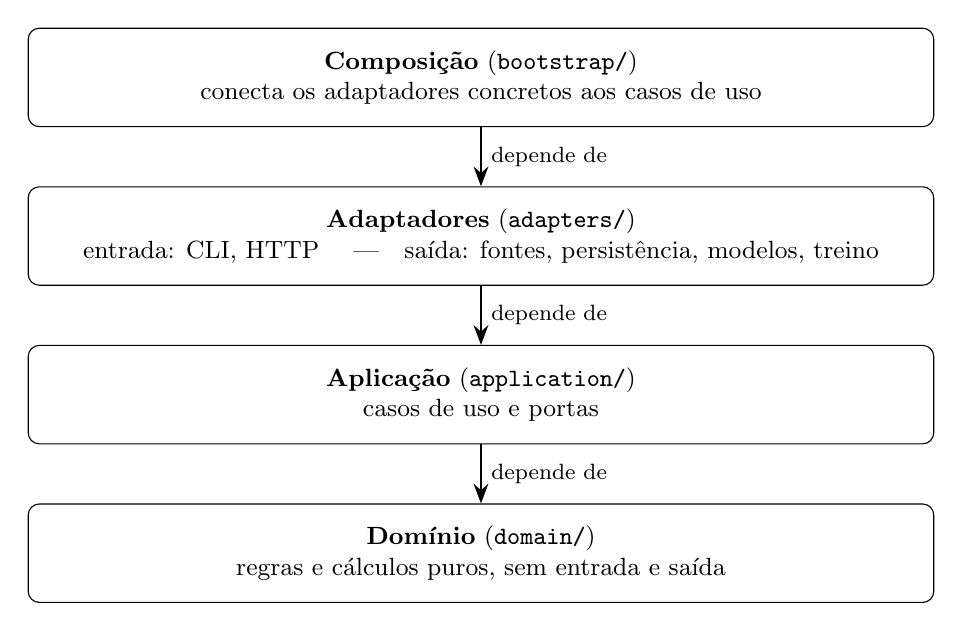
\begin{tikzpicture}[
      caixa/.style={draw, rounded corners, minimum width=11.5cm, minimum height=1.25cm, align=center, font=\small},
      seta/.style={-{Stealth[length=2.5mm]}, thick},
      node distance=0.75cm]
    \node[caixa] (boot) {\textbf{Composição} (\texttt{bootstrap/})\\ conecta os adaptadores concretos aos casos de uso};
    \node[caixa, below=of boot] (adap) {\textbf{Adaptadores} (\texttt{adapters/})\\ entrada: CLI, HTTP \quad|\quad saída: fontes, persistência, modelos, treino};
    \node[caixa, below=of adap] (app) {\textbf{Aplicação} (\texttt{application/})\\ casos de uso e portas};
    \node[caixa, below=of app] (dom) {\textbf{Domínio} (\texttt{domain/})\\ regras e cálculos puros, sem entrada e saída};
    \draw[seta] (boot) -- node[right, font=\footnotesize] {depende de} (adap);
    \draw[seta] (adap) -- node[right, font=\footnotesize] {depende de} (app);
    \draw[seta] (app) -- node[right, font=\footnotesize] {depende de} (dom);
  \end{tikzpicture}
  \legend{Fonte: elaborado pelo autor a partir de \cod{codigo/lazylabel/docs/architecture/clean-hexagonal.md}.}
\end{figure}

\begin{itemize}
  \item \textbf{Domínio} (\cod{src/lazylabel/domain/}). Valores, validações e cálculos independentes de bibliotecas externas, de rede e de arquivos. Está dividido em análise, rotulagem, monitoramento, projetos e treino. É aqui que ficam a política de rotulagem, a decisão entre aplicado e quarentena, a divisão em partições, o ajuste do calibrador, as métricas e as regras de promoção.
  \item \textbf{Aplicação} (\cod{src/lazylabel/application/}). Os casos de uso orquestram o trabalho e declaram \emph{portas}, isto é, protocolos que descrevem o que a aplicação precisa de fontes, persistência, modelos e treino. Os casos de uso recebem suas dependências prontas e não criam adaptadores.
  \item \textbf{Adaptadores} (\cod{src/lazylabel/adapters/}). Os de entrada traduzem argumentos da CLI e requisições HTTP em chamadas à aplicação. Os de saída implementam as portas: leitura de CSV e SQLite, arquivos do \emph{workspace}, modelos locais (Transformers) e treino (PEFT/LoRA).
  \item \textbf{Composição} (\cod{src/lazylabel/bootstrap/}). É a única camada que escolhe e conecta implementações concretas.
\end{itemize}

O painel repete a mesma organização no navegador: as telas consomem uma porta tipada, implementada por um cliente HTTP em produção e por um cliente em memória nos testes.

Para acrescentar uma fonte de dados, por exemplo, define-se a capacidade de leitura na porta de fontes, implementa-se o conector entre os adaptadores de saída e registra-se a escolha na composição. O domínio e os casos de uso não mudam. É essa propriedade que o estudo E2 põe à prova do ponto de vista do usuário: mudar de base sem tocar em \cod{src/}.

\section{Fluxo de uso}
\label{sec:fluxo}

A \autoref{fig:fluxo} resume o fluxo, e as subseções seguintes descrevem cada passo em linguagem simples.

\begin{figure}[htb]
  \centering
  \caption{Fluxo de uso do LazyLabel}
  \label{fig:fluxo}
  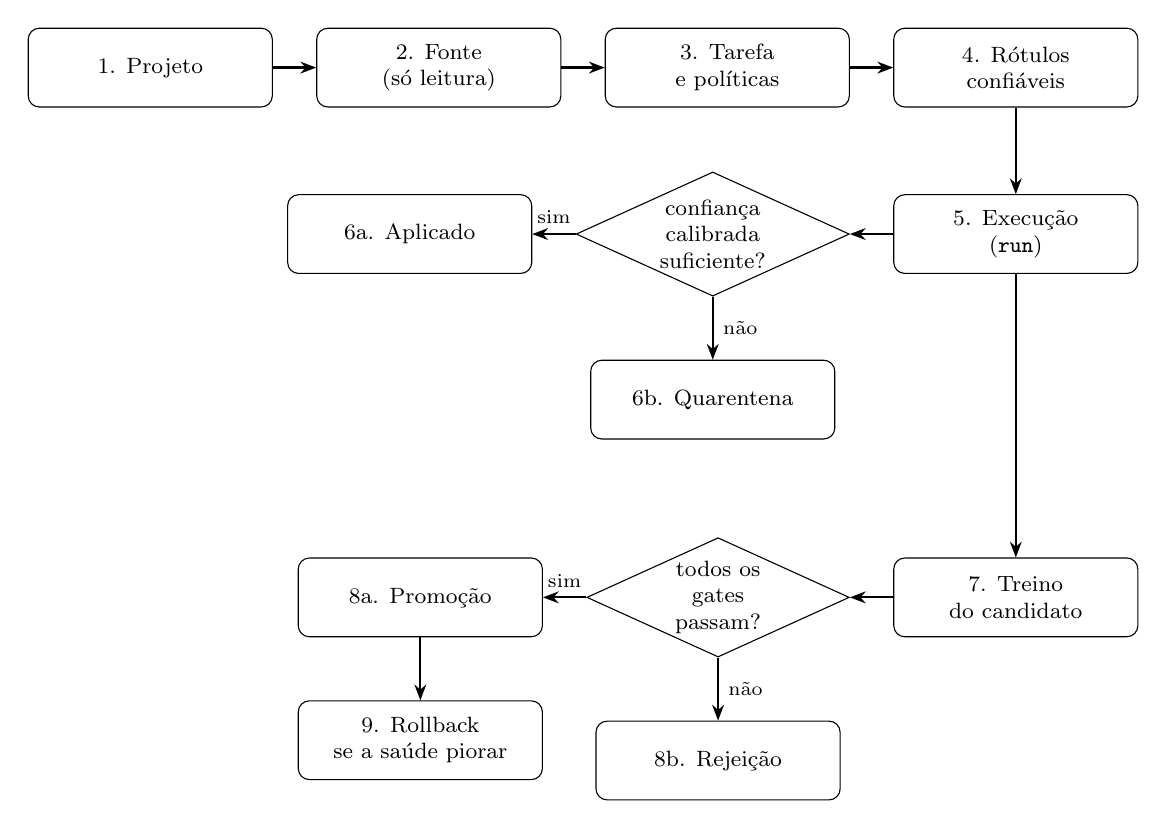
\begin{tikzpicture}[
      passo/.style={draw, rounded corners, minimum width=3.1cm, minimum height=1cm, align=center, font=\footnotesize},
      dec/.style={draw, diamond, aspect=2.2, align=center, font=\footnotesize, inner sep=1pt},
      seta/.style={-{Stealth[length=2mm]}, thick},
      node distance=0.6cm and 0.55cm]
    \node[passo] (proj) {1. Projeto};
    \node[passo, right=of proj] (fonte) {2. Fonte\\(só leitura)};
    \node[passo, right=of fonte] (tarefa) {3. Tarefa\\e políticas};
    \node[passo, right=of tarefa] (conf) {4. Rótulos\\confiáveis};
    \node[passo, below=1.1cm of conf] (run) {5. Execução\\(\texttt{run})};
    \node[dec, left=of run] (ok) {confiança\\calibrada\\suficiente?};
    \node[passo, left=of ok] (apl) {6a. Aplicado};
    \node[passo, below=0.8cm of ok] (quar) {6b. Quarentena};
    \node[passo, below=3.6cm of run] (treino) {7. Treino\\do candidato};
    \node[dec, left=of treino] (gate) {todos os\\gates\\passam?};
    \node[passo, left=of gate] (prom) {8a. Promoção};
    \node[passo, below=0.8cm of gate] (rej) {8b. Rejeição};
    \node[passo, below=0.8cm of prom] (roll) {9. Rollback\\se a saúde piorar};
    \draw[seta] (proj) -- (fonte);
    \draw[seta] (fonte) -- (tarefa);
    \draw[seta] (tarefa) -- (conf);
    \draw[seta] (conf) -- (run);
    \draw[seta] (run) -- (ok);
    \draw[seta] (ok) -- node[above, font=\scriptsize] {sim} (apl);
    \draw[seta] (ok) -- node[right, font=\scriptsize] {não} (quar);
    \draw[seta] (run) -- (treino);
    \draw[seta] (treino) -- (gate);
    \draw[seta] (gate) -- node[above, font=\scriptsize] {sim} (prom);
    \draw[seta] (gate) -- node[right, font=\scriptsize] {não} (rej);
    \draw[seta] (prom) -- (roll);
  \end{tikzpicture}
  \legend{Fonte: elaborado pelo autor.}
\end{figure}

\subsection{Projeto}

O usuário cria uma pasta de trabalho com \cod{lazylabel project init}. Tudo o que a biblioteca produz (configuração, execuções, modelos, partições) fica dentro dela, no diretório \cod{.lazylabel/}. Essa pasta é a fronteira de confiança: os \emph{hashes} gravados detectam alterações acidentais ou externas, mas não protegem contra o próprio dono da pasta.

\subsection{Fonte}

Uma fonte é um arquivo CSV ou uma tabela SQLite, registrada com \cod{lazylabel source add-csv} ou \cod{source add-sqlite}. A fonte é sempre aberta somente para leitura. Os tipos de data e de número são mapeados à mão pelo usuário. É possível capturar o esquema esperado (colunas, tipos, limites de valores ausentes) e, mais tarde, comparar a fonte atual com ele (\cod{lazylabel monitor}).

\subsection{Tarefa e políticas}

Uma tarefa é um arquivo JSON que declara as instruções, as colunas de entrada, os rótulos permitidos e o modelo. O modelo só vê as colunas listadas. A tarefa aponta para uma \emph{política de rotulagem}, que define as regras que todo registro precisa satisfazer (por exemplo, valor não negativo), o limite mínimo de confiança calibrada e o tempo máximo entre a inferência e a decisão. A política não aceita código nem expressões, apenas quatro operadores fixos. Nenhum limite é presumido pela biblioteca: sem política, nada é aplicado.

\subsection{Rótulos confiáveis}

Para treinar e avaliar, o usuário registra uma coluna de referência com \cod{lazylabel supervision add}, informando a proveniência e o tipo de confiança (\cod{provided_ground_truth} ou \cod{validated_rule}) e, se necessário, um mapeamento entre os valores da fonte e os rótulos da tarefa. Esses são os \emph{rótulos confiáveis}: o único alvo permitido para treino e avaliação. A biblioteca valida formato, mapeamento e origem, mas a proveniência é uma declaração do operador. A coluna de rótulo não pode estar entre as colunas de entrada da tarefa.

\subsection{Execução}

O comando \cod{lazylabel run} faz uma rodada de rotulagem seguida do ciclo de treino. Antes de treinar, a biblioteca exige o \emph{gate de treino}, um arquivo (\cod{training-gate.json}) em que o usuário declara modelo, licença, hardware, política de dados e protocolo de avaliação e autoriza explicitamente o treino, e o \emph{gate de promoção}, uma política por tarefa com métricas mínimas, cobertura mínima, regressão máxima por rótulo, erro de calibração máximo, limites de rollback e tamanho mínimo do \emph{holdout}. Se algum pré-requisito falta, o ciclo fica \emph{bloqueado}: nada é treinado nem promovido.

\subsection{Aplicado ou quarentena}

Cada registro termina em um de dois estados. É \emph{aplicado} quando a saída do modelo é válida, as regras da política são satisfeitas, a fonte não mudou desde a leitura e a confiança calibrada atinge o limite. Em qualquer outro caso vai para \emph{quarentena}, com um código de motivo, por exemplo: saída inválida (\cod{invalid_output}), rótulo fora da tarefa (\cod{unknown_label}), regra violada (\cod{rule_conflict}), ausência de calibrador (\cod{uncalibrated}), confiança abaixo do limite (\cod{below_threshold}) ou fonte alterada (\cod{stale_source}). Um registro em quarentena não recebe rótulo e não exige revisão humana; ele apenas conta contra a cobertura.

A confiança usada é sempre a do calibrador. Uma confiança que o modelo declare no próprio texto é rejeitada. Como o calibrador só existe depois que um modelo é avaliado e promovido, na primeira execução de um projeto todas as previsões ficam em quarentena com o motivo \cod{uncalibrated}.

\subsection{Treino com gates}

O ciclo de treino (i) valida a fonte de rótulos confiáveis; (ii) congela partições disjuntas de treino, calibração e \emph{holdout}, gravadas com \emph{hash} e reconstruídas e comparadas byte a byte em execuções posteriores; (iii) treina um candidato com LoRA só na partição de treino; (iv) ajusta um calibrador para cada modelo na partição de calibração; e (v) avalia candidato e incumbente no mesmo \emph{holdout}. Antes da primeira promoção, o incumbente é o modelo-base exato da tarefa.

O calibrador é um artefato imutável, ligado à tarefa, à política, ao modelo exato e ao método de pontuação. Mudar qualquer um desses elementos invalida o calibrador, e as previsões voltam para quarentena.

\subsection{Promoção, rejeição e rollback}

O candidato é \emph{promovido} somente se todos os gates passam: métricas mínimas, cobertura mínima, erro de calibração máximo, ausência de regressão por rótulo acima do permitido e \emph{holdout} com tamanho suficiente. A promoção troca o ponteiro do modelo ativo e grava um evento encadeado por \emph{hash} no registro de modelos. Se algum gate falha, o candidato é \emph{rejeitado}, o modelo ativo permanece e o motivo é registrado. Não existe botão manual de promoção. Depois de uma promoção, se a saúde do modelo violar os limites de rollback, a biblioteca volta automaticamente à versão anterior verificada.

Os comandos \cod{lazylabel run-status} e \cod{lazylabel model-status} mostram o resultado: contagens de aplicados e de quarentenas, motivos, estado do treino, ação de promoção e histórico do modelo, sempre depois de conferir os \emph{hashes} dos artefatos.

\section{Painel}

O comando \cod{lazylabel serve} abre um painel web local, servido em \cod{127.0.0.1}, com checagem de Host, Origin e CSRF. São seis telas: Visão geral, Perguntar, Análises, Monitoramento, Rotulagem e Treinamento. Cada tela é descrita por um arquivo JSON e renderizada por componentes prontos, de modo que alterar uma tela é editar o seu arquivo.

O painel mostra estados agregados (cobertura, motivos de quarentena, histórico de promoção, rejeição e rollback) e não oferece controles por registro, em coerência com a decisão de não haver revisão linha a linha. Na tela Perguntar, o usuário faz uma pergunta sobre uma fonte, revisa o plano de análise proposto, o LazyLabel calcula os números de forma exata e um modelo de linguagem apenas monta a apresentação; telas que contenham números que não vieram do cálculo são descartadas. \pendente{incluir capturas de tela do painel}.

\section{Decisões de projeto}
\label{sec:decisoes}

As decisões que moldaram a biblioteca estão registradas, com motivo e custo, em \cod{tcc/decisoes.md}. O \autoref{qua:decisoes} as resume.

\begin{quadro}[htb]
  \caption{Decisões de projeto}
  \label{qua:decisoes}
  \small
  \begin{tabularx}{\textwidth}{|c|X|X|}
    \hline
    \textbf{N.º} & \textbf{Decisão} & \textbf{Motivo e custo} \\ \hline
    1 & Tudo roda na máquina do usuário; nenhum dado sai dela. Substituída pela decisão 8; o modo local continua como opção. & Dados financeiros são sensíveis. Custo: qualidade limitada a modelos leves. \\ \hline
    2 & Fontes CSV e SQLite abertas só para leitura. & Ler sem risco de alterar. Custo: não escreve de volta; só dois tipos de fonte. \\ \hline
    3 & Código em camadas, com o domínio no centro. & Trocar modelo, fonte ou interface sem reescrever regras. Custo: mais arquivos. \\ \hline
    4 & Rotulagem autônoma: cada registro é aplicado ou vai para quarentena. & Ninguém revisa linha a linha; na dúvida, o sistema se abstém. Custo: sem calibrador, tudo vai para quarentena na primeira execução. \\ \hline
    5 & Treino só com rótulos confiáveis; promoção só se todos os gates passam; rollback automático. & Trocar de modelo só com evidência e poder voltar atrás. Custo: exige configurar autorização, políticas e rótulos antes do treino. \\ \hline
    6 & Análises calculadas de forma exata, com aritmética decimal, a partir de um plano revisável. & Números financeiros não podem variar por arredondamento ou pelo modelo. Custo: só operações simples. \\ \hline
    7 & O tema do TCC passa a ser a biblioteca, avaliada por reutilização. & Define a pergunta de pesquisa deste trabalho. \\ \hline
    8 & Modelos na nuvem por um \emph{gateway} de modelos e painel descrito em JSON. & Autorizada em 09/11/2026. A rotulagem continua local, pois a calibração precisa da pontuação de cada rótulo. \\ \hline
    9 & Desenho final do experimento, fixado em 10/11/2026 antes dos resultados. & Baseline, comparação entre modelo-base e ajustado, segunda base, correções no núcleo antes do congelamento e rótulo pela pontuação. \\ \hline
  \end{tabularx}
  \legend{Fonte: \cod{tcc/decisoes.md}.}
\end{quadro}

Duas dessas decisões merecem comentário. A decisão~1 foi substituída pela~8: o envio de dados à nuvem deixou de ser proibido, mas o que sustentava a decisão original continua valendo no fluxo de rotulagem, isto é, o modelo recebe só as colunas da tarefa, os \emph{logs} não guardam linhas e a ausência de confiança calibrada leva à quarentena. Nos experimentos deste trabalho, toda a rotulagem e todo o treino foram locais.

A decisão~9 inclui uma mudança motivada por evidência. Em um teste preliminar com o modelo-base em 50 registros de desenvolvimento, o rótulo escrito pelo modelo no texto gerado discordava do rótulo de maior pontuação em 34\% dos casos (\autoref{sec:fumaca}). Como a calibração é feita sobre a pontuação, essa divergência faria o ciclo abortar. A partir daí, o rótulo previsto passou a ser, por definição, o de maior verossimilhança, e a geração de texto serve apenas para validar o formato.

\section{Testes}

A biblioteca tem testes automatizados em quatro grupos: testes de domínio e de aplicação, testes dos adaptadores, testes de ponta a ponta da CLI e do painel, e um teste de arquitetura (\cod{tests/architecture/test_layer_dependencies.py}) que falha se alguma camada importar código de uma camada externa a ela. O painel tem testes próprios e verificação de tipos. Um único comando, \cod{bash factory/checks.sh}, executa todas as verificações.

Em 09/11/2026, o arquivo \cod{README.md} do repositório registrava 340 testes em Python e 57 testes do painel passando. \pendente{reexecutar \cod{bash factory/checks.sh} no commit final e atualizar as contagens}.

Os testes do ciclo de treino usam um modelo substituto (\emph{stub}), para não depender de pesos reais nem de hardware específico. Por isso, eles verificam as regras do ciclo (bloqueio, promoção, rejeição, rollback, integridade dos artefatos), mas não a qualidade de um modelo real. Essa segunda verificação é o papel dos experimentos do \autoref{cap:resultados}.

\chapter{Resultados e discussão}
\label{cap:resultados}

% RASCUNHO: este capítulo é ESTRUTURA. Só aparecem números que já estão
% registrados em arquivos do repositório (citados em cada seção). Tudo o que
% depende do teste final está marcado com \pendente{...}.

Este capítulo apresenta primeiro os resultados preliminares, obtidos antes de abrir qualquer teste final, e depois os resultados dos estudos E1 e E2. \pendente{os resultados do E1 e do E2 ainda não foram obtidos; as seções correspondentes contêm apenas a estrutura}.

\section{Resultados preliminares}

\subsection{Experimento sintético}

Antes dos dados reais, a cadeia técnica (exportar exemplos, ajustar um adapter LoRA, recarregá-lo e inferir) foi verificada em dados sintéticos: descrições financeiras geradas por moldes de frase (\emph{templates}), classificadas em três categorias, com 72 exemplos de treino e 24 reservados. O ajuste usou posto 8, três épocas, lote 1, taxa de aprendizado $2\times10^{-4}$ e semente 42. A \autoref{tab:sintetico} traz o resultado nos 24 exemplos reservados.

\begin{table}[htb]
  \centering
  \caption{Experimento sintético: modelo-base e adapter LoRA nos 24 exemplos reservados}
  \label{tab:sintetico}
  \begin{tabular}{lcc}
    \toprule
    Métrica & Modelo-base & Com adapter LoRA \\
    \midrule
    Acurácia exata & 9/24 (37,5\%) & 17/24 (70,8\%) \\
    Macro-F1 & 0,300 & 0,706 \\
    Saídas válidas & 23/24 (95,8\%) & 24/24 (100\%) \\
    \bottomrule
  \end{tabular}
  \legend{Fonte: \cod{tcc/experimentos/sintetico-qwen-0.5b/RESULTS.md}.}
\end{table}

Esse resultado mostra apenas que a cadeia funciona. A amostra é pequena e artificial, os rótulos foram gerados por regras, e treino e avaliação compartilham vocabulário e padrões; nada disso permite concluir qualidade em dados reais. Além disso, o experimento é anterior ao fluxo autônomo atual: o adapter produzido não tem calibrador e não pode ser promovido pelo ciclo descrito no \autoref{cap:desenvolvimento}.

\subsection{Teste de fumaça do modelo-base}
\label{sec:fumaca}

Em 10/11/2026, antes do congelamento da configuração do E1, o modelo-base sem ajuste foi executado nos 50 primeiros registros do conjunto de desenvolvimento da South German Credit, para medir a taxa de saídas válidas (\autoref{tab:fumaca}). O teste final não foi usado, e não houve medida de acerto.

\begin{table}[htb]
  \centering
  \caption{Teste de fumaça do modelo-base em 50 registros de desenvolvimento}
  \label{tab:fumaca}
  \small
  \begin{tabular}{lcccc}
    \toprule
    Rodada & Saídas válidas & Rótulo igual ao vencedor & Previstos & Tempo \\
    & & por pontuação & (\texttt{good}/\texttt{bad}) & \\
    \midrule
    1 (rótulo gerado) & 50/50 & 33/50 & 22/28 & 28 s \\
    2 (rótulo = vencedor) & 50/50 & 50/50 & 39/11 & 29 s \\
    \bottomrule
  \end{tabular}
  \legend{Fonte: \cod{tcc/experimentos/sgc-real/fumaca-2026-11-10.md}.}
\end{table}

Na primeira rodada, o rótulo escrito no texto gerado discordava do rótulo de maior pontuação em 17 dos 50 casos (34\%). Como a calibração opera sobre a pontuação, o ciclo abortaria. Esse achado levou à regra, registrada na decisão~9, de que o rótulo previsto é o de maior verossimilhança.

\subsection{Baseline por validação cruzada no desenvolvimento}

A \autoref{tab:baseline-cv} traz as médias da validação cruzada de cinco partições do baseline, calculadas só nos 800 registros de desenvolvimento de cada base. O teste final permanecia fechado quando esses números foram registrados.

\begin{table}[htb]
  \centering
  \caption{Baseline (regressão logística): média da validação cruzada no desenvolvimento}
  \label{tab:baseline-cv}
  \begin{tabular}{lcc}
    \toprule
    Métrica & South German Credit & Default of Credit Card Clients \\
    \midrule
    Acurácia & 0,744 & 0,816 \\
    Macro-F1 & 0,678 & 0,688 \\
    Brier (\emph{top-label}) & 0,170 & 0,137 \\
    ECE (\emph{top-label}, 10 faixas) & 0,080 & 0,049 \\
    \bottomrule
  \end{tabular}
  \legend{Fonte: \cod{resultados/baseline/baseline.json} em \cod{tcc/experimentos/sgc-real/} e em \cod{tcc/experimentos/default-real/}.}
\end{table}

Para referência, prever sempre a classe majoritária acerta 70,0\% na primeira base e 77,9\% na amostra da segunda. Na segunda base, portanto, a acurácia do baseline fica poucos pontos acima da taxa-base, e o macro-F1 é a medida mais informativa. Esses números são de desenvolvimento e servem apenas para dimensionar a comparação; os resultados válidos para as hipóteses são os do teste final.

\section{E1: qualidade na South German Credit}

\subsection{Ciclo de treino e promoção}

\pendente{resultado do ciclo \cod{lazylabel run} no desenvolvimento: tamanho real das partições de treino, calibração e holdout; métricas do candidato e do incumbente no holdout interno; quais gates passaram; ação final (promoção, rejeição ou bloqueio); tempo de treino; saídas de \cod{run-status} e \cod{model-status}}.

\subsection{Teste final}

\pendente{data e commit da abertura única do teste final}.

\begin{table}[htb]
  \centering
  \caption{E1: resultados no teste final (200 registros)}
  \label{tab:e1}
  \begin{tabular}{lccc}
    \toprule
    Métrica & Baseline (todos) & Baseline (só aplicados) & LazyLabel \\
    \midrule
    Acurácia & \pendente{} & \pendente{} & \pendente{} \\
    Macro-F1 & \pendente{} & \pendente{} & \pendente{} \\
    Brier (\emph{top-label}) & \pendente{} & \pendente{} & \pendente{} \\
    ECE (\emph{top-label}) & \pendente{} & \pendente{} & \pendente{} \\
    Cobertura & 100\% & -- & \pendente{} \\
    \bottomrule
  \end{tabular}
  \legend{Fonte: \pendente{arquivo de resultados do E1}.}
\end{table}

\pendente{intervalos de confiança por bootstrap pareado (1000 reamostragens) para as diferenças principais}.

\pendente{figura: curva de risco por cobertura do baseline, com o ponto do LazyLabel marcado}.

\pendente{tabela: matriz de confusão do LazyLabel nos registros aplicados}.

\pendente{tabela: contagem de quarentenas por motivo}.

\subsection{Discussão das hipóteses}

\begin{description}
  \item[H1.] \pendente{diferença de acurácia entre o LazyLabel nos aplicados e o baseline na mesma cobertura; dizer se ficou dentro dos 5 pontos percentuais e com que intervalo}.
  \item[H2.] \pendente{houve promoção? cobertura no teste e comparação com o mínimo de 0,10}.
  \item[H3.] \pendente{ECE e Brier do LazyLabel em todas as previsões do teste, comparados aos do baseline e ao limite de 0,12}.
\end{description}

\pendente{se houver, comparação com o modelo-base calibrado sem ajuste (efeito do ajuste fino)}.

\section{E2: reutilização na Default of Credit Card Clients}

\subsection{O que mudou}

Até a preparação do E2, a comparação entre as configurações dos dois estudos (arquivo \cod{tcc/experimentos/default-real/alteracoes-config.diff}) mostra alterações apenas em arquivos de configuração: na tarefa, as instruções e as colunas de entrada; na política de rotulagem, os campos das regras; e no gate de treino, a descrição da política de dados. Nenhum arquivo em \cod{codigo/lazylabel/src/} foi alterado. Essa constatação vale para a preparação; \pendente{confirmar, depois de rodar o ciclo e o teste do E2, se alguma mudança de código foi necessária, e anexar o \cod{git diff} correspondente}.

\begin{quadro}[htb]
  \caption{E2: alterações em relação ao E1}
  \label{qua:e2-alteracoes}
  \small
  \begin{tabularx}{\textwidth}{|X|X|X|}
    \hline
    \textbf{Item} & \textbf{Só configuração} & \textbf{Exigiu mudar código} \\ \hline
    Tarefa (instruções, colunas de entrada) & Sim & \pendente{} \\ \hline
    Política de rotulagem (regras) & Sim & \pendente{} \\ \hline
    Gate de treino (política de dados) & Sim & \pendente{} \\ \hline
    Política de promoção & Sem alteração & \pendente{} \\ \hline
    Mapeamento de rótulos e tipos de coluna & \pendente{} & \pendente{} \\ \hline
    Execução do ciclo e do teste & \pendente{} & \pendente{} \\ \hline
  \end{tabularx}
  \legend{Fonte: \cod{tcc/experimentos/default-real/alteracoes-config.diff} e \pendente{registro da execução do E2}.}
\end{quadro}

\pendente{tabela: passos executados no E2 e tempo de cada um}.

\subsection{Qualidade na segunda base}

\begin{table}[htb]
  \centering
  \caption{E2: resultados no teste final (200 registros)}
  \label{tab:e2}
  \begin{tabular}{lccc}
    \toprule
    Métrica & Baseline (todos) & Baseline (só aplicados) & LazyLabel \\
    \midrule
    Acurácia & \pendente{} & \pendente{} & \pendente{} \\
    Macro-F1 & \pendente{} & \pendente{} & \pendente{} \\
    Brier (\emph{top-label}) & \pendente{} & \pendente{} & \pendente{} \\
    ECE (\emph{top-label}) & \pendente{} & \pendente{} & \pendente{} \\
    Cobertura & 100\% & -- & \pendente{} \\
    \bottomrule
  \end{tabular}
  \legend{Fonte: \pendente{arquivo de resultados do E2}.}
\end{table}

\pendente{resultado do ciclo de treino e promoção no E2, intervalos por bootstrap e contagem de quarentenas por motivo}.

\section{Discussão geral}

\pendente{resposta à pergunta de pesquisa à luz do E1 e do E2: até que ponto o fluxo foi reaplicado sem alterar o núcleo; o que a rastreabilidade registrou; o que o controle de qualidade (quarentena e gates) impediu ou permitiu}.

\pendente{discutir o custo: tempo de treino e de inferência do modelo de linguagem em comparação com o baseline, e se o resultado justifica um modelo de linguagem em dados tabulares}.

\pendente{ameaças à validade observadas na execução (por exemplo, necessidade de repetir alguma etapa)}.

\chapter{Conclusão}
\label{cap:conclusao}

% RASCUNHO: este capítulo é ESTRUTURA. As conclusões dependem dos resultados
% do Capítulo 5 e devem ser escritas pelo autor depois de obtê-los.

Este trabalho propôs e implementou o LazyLabel, uma biblioteca de rotulagem autônoma de dados financeiros tabulares em que um rótulo só é aplicado com confiança calibrada suficiente, os demais registros vão para quarentena, e um modelo ajustado só substitui o anterior quando passa em todos os gates de promoção. A pergunta de pesquisa era até que ponto esse fluxo configurável pode ser reaplicado a outras tarefas e bases sem alterar o núcleo, mantendo rastreabilidade e controle de qualidade.

\section{Síntese dos resultados}

\pendente{um parágrafo com a resposta à pergunta de pesquisa}.

\pendente{E1: o que se concluiu sobre H1, H2 e H3, com os números principais e seus intervalos}.

\pendente{E2: o que mudou só em configuração e o que exigiu mudar código}.

\section{Atendimento aos objetivos}

\pendente{retomar cada objetivo específico do \autoref{cap:introducao} e dizer, com base nos capítulos anteriores, se foi atendido, parcialmente atendido ou não atendido}.

\section{Limitações}

Algumas limitações são conhecidas desde o desenho do trabalho e independem dos resultados:

\begin{itemize}
  \item as duas bases são públicas, antigas e de outros países, e não representam carteiras brasileiras atuais;
  \item os conjuntos de teste têm 200 registros, o que produz intervalos de confiança largos;
  \item as duas bases pertencem ao mesmo domínio e têm alvo binário, de modo que a reutilização foi medida em um caso próximo do original;
  \item a biblioteca lê apenas CSV e SQLite, e a rotulagem depende de um modelo local que forneça a pontuação de cada rótulo;
  \item não houve avaliação de usabilidade com usuários;
  \item os \emph{hashes} gravados garantem integridade dentro da pasta do projeto, mas não autenticam quem produziu os rótulos confiáveis.
\end{itemize}

\pendente{limitações observadas na execução dos experimentos}.

\section{Trabalhos futuros}

\begin{itemize}
  \item Calibração como passo explícito, separado do treino, para que o primeiro uso de um projeto não termine com cobertura zero (opção~C da pergunta~8 em \cod{tcc/perguntas-orientador.md}).
  \item Rotulagem com modelos em nuvem, o que depende de obter, do serviço, a pontuação de cada rótulo.
  \item Repetição dos experimentos com várias sementes, para medir a variabilidade do treino.
  \item Aplicação a uma base de outro domínio e a uma tarefa com mais de duas classes.
  \item Novas fontes de dados, implementadas como adaptadores.
\end{itemize}

\pendente{o autor deve rever esta lista depois dos resultados e da conversa com o orientador}.


% ---------------------------------------------------------------------------
% ELEMENTOS PÓS-TEXTUAIS
% ---------------------------------------------------------------------------
\postextual

\bibliography{referencias}

\begin{apendicesenv}
\partapendices
\chapter{Declaração de uso de inteligência artificial}
\label{ap:uso-de-ia}

Este apêndice declara como ferramentas de inteligência artificial (IA) generativa foram usadas neste trabalho. Ele se baseia no acordo de trabalho registrado no arquivo \cod{tcc/uso-de-ia.md} do repositório do projeto.

\section{Autorização e princípios}

Em 19/10/2026, o autor informou ter conversado com o professor e recebido autorização para usar IA como apoio no TCC, com o objetivo de otimizar o tempo. \pendente{confirmar com o orientador quais usos específicos são aceitos e como devem ser declarados; registrar a data da confirmação}. A Universidade Federal de Uberlândia publicou recomendações de uso ético e responsável de IA, que orientam supervisão humana, transparência, privacidade e registro quando necessário para validação ou reprodução\footnote{Portaria REITO n.º 539/2026, conforme citada em \cod{tcc/uso-de-ia.md}. \pendente{o autor deve conferir o número, a data e o texto da portaria na fonte oficial antes de mantê-la aqui}.}.

Os princípios adotados foram: a IA pode acelerar tarefas de pesquisa e de execução, mas não substitui as decisões, a análise nem a responsabilidade do autor; referências sugeridas por IA só são usadas depois de conferidas na fonte original; texto ou código produzido por IA não é comprovação de resultado; e só dados públicos ou sintéticos foram compartilhados com as ferramentas.

\section{Como a IA foi usada}

\begin{itemize}
  \item \textbf{Texto da monografia.} A primeira versão deste documento foi redigida com assistência do Claude, um modelo de linguagem da Anthropic, usado pela ferramenta Claude Code, a partir dos documentos do repositório (decisões, protocolo, plano do experimento, documentação do código e registros dos experimentos). O autor revisou o texto, conferiu as afirmações e as referências e reescreveu o conteúdo. \pendente{o autor deve confirmar esta frase depois de concluir a revisão e indicar a versão do modelo usada}.
  \item \textbf{Código.} O código do LazyLabel e os roteiros dos experimentos foram desenvolvidos com assistência de agentes de programação baseados em modelos de linguagem. As alterações passaram por testes automatizados e por revisão antes de serem incorporadas. \pendente{o autor deve descrever a extensão desse uso e nomear as ferramentas e versões, a partir do histórico do repositório}.
  \item \textbf{Protocolo e decisões.} A IA foi usada para organizar decisões, redigir e revisar o protocolo experimental e apontar riscos de vazamento. As hipóteses, os limiares e as escolhas de base e de baseline são de responsabilidade do autor e estão sujeitas à aprovação do orientador.
  \item \textbf{Estudo e literatura.} A IA foi usada para explicar conceitos e sugerir termos de busca e referências. \pendente{o autor deve confirmar que leu e conferiu cada referência citada; as entradas marcadas com VERIFICAR no arquivo de referências ainda têm dados a conferir}.
\end{itemize}

\section{O que não foi delegado}

Os resultados numéricos deste trabalho vêm da execução dos programas sobre os dados e estão registrados em arquivos do repositório; nenhum número foi produzido por um modelo de linguagem. A interpretação dos resultados e as conclusões são do autor.

\section{Registro de uso}

O \autoref{qua:registro-ia} é o registro resumido dos usos relevantes, no formato previsto em \cod{tcc/uso-de-ia.md}. \pendente{preencher; o registro no repositório estava vazio quando este rascunho foi gerado}.

\begin{quadro}[htb]
  \caption{Registro de uso de IA}
  \label{qua:registro-ia}
  \small
  \begin{tabularx}{\textwidth}{|p{1.9cm}|>{\raggedright\arraybackslash}p{2.2cm}|>{\raggedright\arraybackslash}X|>{\raggedright\arraybackslash}X|>{\raggedright\arraybackslash}X|}
    \hline
    \textbf{Data} & \textbf{Ferramenta} & \textbf{Tarefa} & \textbf{O que foi aproveitado} & \textbf{Como foi validado} \\ \hline
    10/11/2026 & Claude (Claude Code) & Rascunho da monografia & Estrutura e primeira redação dos capítulos & \pendente{revisão do autor} \\ \hline
    \multicolumn{5}{|l|}{\pendente{demais usos, uma linha por uso relevante}} \\ \hline
  \end{tabularx}
  \legend{Fonte: elaborado pelo autor.}
\end{quadro}

\end{apendicesenv}

\end{document}
